% ====== TAREA 1 DE PROBABILIDAD ======

\documentclass[12pt,a4paper]{report}
\usepackage[utf8x]{inputenc}
\usepackage{amsmath}
\usepackage{amsfonts}
\usepackage{amssymb}
\usepackage{graphicx}
\usepackage{enumitem}
\usepackage{calrsfs}

\newcommand*{\Comb}[2]{{}^{#1}C_{#2}}

\begin{document}
\begin{titlepage}
	\centering
	{\scshape\LARGE Universidad Autónoma de México \par}
	\vspace{1cm}
	{\scshape\Large Probabilidad I\par}
	\vspace{1.5cm}
	{\huge\bfseries Tarea I\par}
	\vspace{.5cm}
	{\Large\itshape Sandra Del Mar Soto Corderi \par}
	\vspace{.5cm}
	{\Large\itshape Edgar Quiroz Castañeda \par}
    \vspace{.5cm}
	{\Large\itshape Raúl Llamosas Alvarado \par}
	 \vspace{.5cm}
	{\Large\itshape Alan Ernesto Arteaga Vázquez \par}
	\vfill
	 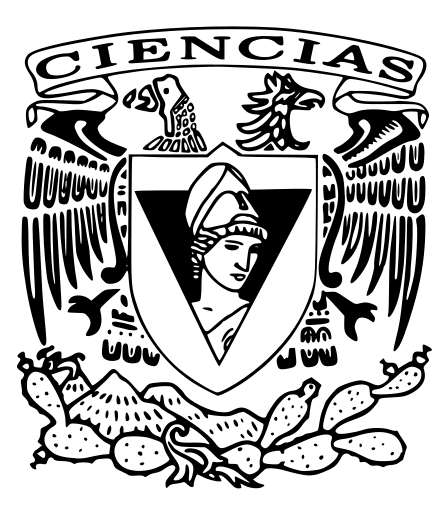
\includegraphics[width=0.5\textwidth]{escudo.png}
	\vfill

% Bottom of the page
	{\large Martes 21 de Agosto del 2018 \par}
\end{titlepage}

\pagebreak
\setlength{\voffset}{-0.75in}
\setlength{\headsep}{5pt}

\begin{enumerate}
   % Ejercicio 1
   \item {
  La diferencia simétrica de dos conjuntos A,B se define como:\\

		$$A\triangle B = (A \cap B^c) \cup (B \cap A^c)=(A \cup B) \setminus (B \cap A)$$
Demuestre
\begin{enumerate}[label=\alph*) ]
	%a
	\item{
		$A^c \triangle B^c = A \triangle B $ \\

		Notemos que tanto la unión como la itersección conmutan, y que el complemento
		del complemento es el conjunto original.\\
		De estas tres cosas y de la definición de diferencia simétrica, tenemos que
		\begin{align*}
			A^c \triangle B^c &= (A^c \cap (B^c)^c)) \cup (B^c \cap (A^c)^c))\\
												&= (A^c \cap B) \cup (B^c \cap A)\\
												&= (B \cap A^c) \cup (A \cap B^c)\\
												&= (A \cap B^c) \cup (B \cap A^c)\\
												&= A \triangle B
		\end{align*}
	}

	%b
	\item{
		$ (A_{1} \cup A_{2})\triangle (B_{1} \cup B_{2})\subseteq (A_{1} \triangle B_{1}) \cup (A_{2} \triangle B_{2}) $ \\

		Sea $x \in (A_{1} \cup A_{2})\triangle (B_{1} \cup B_{2})
		= ((A_{1} \cup A_{2}) \cap (B_{1} \cup B_{2})^c) \cup ((B_{1} \cup B_{2}) \cap (A_{1} \cup A_{2})^c)$.\\
		Esto es, que $x \in (A_{1} \cup A_{2})$ o $x \in (B_{1} \cup B_{2})$,
		pero no los dos al mismo tiempo.\\
		Primero veamos que pasa si $x \in (A_{1} \cup A_{2})$.\\
		Entonces $x \notin (B_{1} \cup B_{2})$ y $x \in A_1$ o  $x \in A_2$.
		Sin perdidad de generalidad, digamos que $x \in A_1$. Entonces en particular
		$x \in (A_1 \cup B_1)$. Además, como $x \notin (B_{1} \cup B_{2})$,
		entonces tenemos que $x \notin B_1$ ni $x \notin B_2$, por lo que en particular
		$x \notin (B_1 \cap A_1)$. Entonces $x \in ((A_1 \cup B_1) \setminus (B_1 \cap A_1)) =
		(A_{1} \triangle B_{1})$.\\
		Analogamente, si $x \in A_2$, tenemos que $x \in (A_2 \triangle B_2)$.\\
		Luego, si $x \in (B_{1} \cup B_{2})$, entonces $x \notin (A_{1} \cup A_{2})$ y
		$x \in B_1$ o  $x \in B_2$.\\
		Como en el caso anterior, si $x \in B_1$, entonces $x \in (B_1 \cup A_1)$ y
		$x \notin (A_1 \cap B_1)$, por lo que $x \in A_{1} \triangle B_{1}$.\\
		Y analogamente, si $x \in B_2$, pasa que $x \in A_2 \triangle B_2$.\\
		Entonces, sin importar el elemento que tomemos de $(A_{1} \cup A_{2})\triangle (B_{1} \cup B_{2})$,
		éste está contenido en $(A_{1} \triangle B_{1}) \cup (A_{2} \triangle B_{2})$.\\
	}

	%c
	\item{
		Sea $\Omega$ un conjunto y $\mathcal{F} \subseteq P(\Omega)$ una $\sigma$-algebra.
		Demuestre que $A \triangle B \in \mathcal{F} $ siempre que $A,B \in \mathcal{F}$. \\\\
		Como $\mathcal{F}$ es una $\sigma$-algebra, entonces es cerrada bajo el complemento y la unión. Entonces
		\begin{align*}
			A,B \in \mathcal{F} &\implies A^c,B^c \in \mathcal{F}\\
													&\implies (A^c \cup B),(B^c \cup A) \in \mathcal{F}\\
													&\implies (A^c \cup B)^c = (A \cap B^c),(B^c \cup A)^c = (B \cap A^c) \in \mathcal{F}\\
													&\implies (A \cap B^c) \cup (B \cap A^c) = A \triangle B \in \mathcal{F}.
		\end{align*}

	}



\end{enumerate}

	}

	% Ejercicio 2
   \item {
    Si $\Omega = \lbrace 1,2,3,4,5 \rbrace$ construya una $\sigma$-álgebra $\mathcal{F} \neq \mathcal{P}(\Omega)$ tal que:\\
    $$\lbrace \lbrace 1,2 \rbrace , \lbrace 1,3 \rbrace \rbrace \subset \mathcal{F}$$

		Se puede construir una $\sigma$-álgebra agregando los elementos faltantes
		para que cumpla los axiomas.\\
		Primero, toda $\sigma$-algebra contiene al vacío y al universo, por lo que
		$\Omega, \emptyset \in \mathcal{F}$.\\
		Faltan además los complementos de los elementos dados, que son $\lbrace 3, 4, 5 \rbrace, \\
		\lbrace 2, 4, 5 \rbrace \in \mathcal{F}$.\\
		Y faltan las uniones de los elementos actuales, que son  $\lbrace 1, 2, 3 \rbrace,
		\lbrace 1, 2, 4, 5 \rbrace, \lbrace 1, 4, 5 \rbrace, \\
		\lbrace 2, 3, 4, 5 \rbrace \in \mathcal{F}$.\\
		Entonces faltarían los complementos de los nuevos eventos, que son
		$\lbrace 4, 5 \rbrace, \lbrace 3 \rbrace, \lbrace 2, 3 \rbrace, \lbrace 1 \rbrace
		\in \mathcal{F}$.\\
		Y nuevamente faltarían las nuevas posibles uniones, que solo es una en este caso.
		$\lbrace 1, 3, 4, 5 \rbrace \in \mathcal{F}$\\
		Y al llegar a este punto, nuestro conjunto ya es cerrado baja la unión y el
		complemento.
		Entonces una $\sigma$-álgebra que cumple lo requierido es\\
		$\mathcal{F} = \lbrace \emptyset,
		\lbrace 3 \rbrace, \lbrace 1 \rbrace,
		\lbrace 4, 5 \rbrace, \lbrace 2, 3 \rbrace, \lbrace 1,2 \rbrace , \lbrace 1,3 \rbrace,
		\lbrace 1, 2, 3 \rbrace, \lbrace 3, 4, 5 \rbrace, \lbrace 2, 4, 5 \rbrace, \lbrace 1, 4, 5 \rbrace, \\
		\lbrace 1, 2, 4, 5 \rbrace, \lbrace 2, 3, 4, 5 \rbrace,
		\Omega \rbrace$
	}


	% Ejercicio 3
   \item {
   En una universidad se ofrecen tres cursos de idiomas: uno  de inglés, uno de francés y otro de alemán.
	 Cualquiera de los 100 alumnos de la escuela puede tomar dichos cursos.
	 Hay 26 estudiantes en la clase de inglés, 28 en la de francés y 16 en la de alemán.
	 Hay 12 estudiantes que están en el de inglés y francés, 4 en el de ingles y alemán ,
	 6 en el de alemán y francés y 2 tomando los tres cursos\\

	 Digamos que I representa a los estudiantes de inglés, F de francés y A de alemán.
	 Entonces las cantidades de alumnos se puede representar como probabilidades.

		\begin{center}
		 \begin{tabular}{|c|c|}
							\hline
							Idioma & Porcentaje  \\
							\hline
							I & 26\% \\
							\hline
							F & 28\% \\
							\hline
							A & 16\% \\
							\hline
							I y F & 12\% \\
							\hline
							I y A & 4\% \\
							\hline
							F y A & 6\% \\
							\hline
							I, F y A & 2\% \\
							\hline
			\end{tabular}
		\end{center}

	\begin{enumerate}[label=\alph*) ]
	% a)
   \item {
		Si un estudiante se selecciona aleatoriamente ¿Cual es la probabilidad de que no esté inscrito en ningún curso de idiomas?\\

		El evento que corresponde a todos los alumnos estudiando idiomas es
		$I \cup F \cup A$, entonces lo contrario, el evento que corresponde a los
		alumnos que no toman ningún idioma, es $(I \cup F \cup A)^c$.
		Entonces
		\begin{align*}
			P((I \cup F \cup A)^c) &= 1 - P(I \cup F \cup A)\\
														 &= 1 - (P(I) + P(F) + P(A) - P(I \cap F))\\
														 &- P(I \cap A) - P(F \cap A) + P(I \cap F \cap A))\\
														 &= 1 - (0.26 + 0.28 + 0.16 - 0.12 - 0.04 - 0.06 + 0.02)\\
														 &= 1 - 0.5\\
														 &= 0.5
		\end{align*}
		Entonces hay una probabilidad de 0.5 de que el alumno elegido no esté tomando ningún idioma.
   }

   % b)
   \item {
   Si un estudiante se selecciona aleatoriamente, ¿Cual es la probabilidad de que lleve exactamente uno de los cursos de idiomas?\\

	 Consideremos primero a los alumnos que sólo estudian inglés.
	 Este evento es $I' = I \setminus (F \cup A)$.
	 Entonces
	 \begin{align*}
	 	P(I') &= P(I \setminus (F \cup A))\\
					&= P(I) - P(I \cap (F \cup A))\\
					&= 0.26 - P((I \cap F) \cup (I \cap A))\\
					&= 0.26 - (P(I \cap F) + P(I \cap A) - P(I \cap A \cap F))\\
					&= 0.26 - (0.12 + 0.04 - 0.02)\\
					&= 0.26 - 0.14\\
					&= 0.12
	 \end{align*}
   }

	 Análogamente, los eventos que corresponden a los alumnos que sólo estudian
	 alemán y francés son $F' = F \setminus (I \cup A)$  y $A' = A \setminus (F \cup I)$.\\
	 Y sus probabilidades son
	 \begin{align*}
	 	P(F') &= P(F) - (P(F \cap I) + P(F \cap A) - P(I \cap A \cap F))\\
					&= 0.28 - (0.12 + 0.06 - 0.02)\\
					&= 0.28 - 0.16\\
					&= 0.12
	 \end{align*}
	 Y
	 \begin{align*}
	 	P(A') &= P(A) - (P(A \cap F) + P(A \cap I) - P(I \cap A \cap F))\\
					&= 0.16 - (0.06 + 0.04 - 0.02)\\
					&= 0.16 - 0.08\\
					&= 0.08
	 \end{align*}

	 Entonces el evento que corresponde a que un estudiante sólo esté inscrito en
	 un idioma es $P(I' \cup F' \cup A')$.\\
	 Estos eventos son ajenos, pues precisamente corresponden a personas
	 estudiando únicamente un idioma, no más.\\
	 Entonces la probabilidad de este evento es
	 $$P(I' \cup F' \cup A') = P(I') + P(F') + P(A') = 0.12 + 0.12 + 0.8 = 0.32$$
	 Entonces hay una probabilidad de 0.32 de que un estudiante seleccionado
	 aleatoriamente estudie sólo un idioma.

    % c)
   \item {
  	Si dos estudiantes se seleccionan aleatoriamente ¿Cual es la probabilidad de que al menos uno esté tomando alguna clase de idiomas?\\

		Llamemos a este evento $A$.\\
		Consideremos el evento contrario, es decir que escogiendo dos personas 
		aleatoriamente, ninguna esté estudiando un idioma.\\
		En el inciso anterior se calculó la probabiliad de no estar estudiando ningún idioma como 0.5.\\ 
		Teniendo en cuenta que hay 100 estudiantes, esto significa 
		50 alumnos que no estudian idiomas.\\
		Entonces la probabilidad de elegir a dos estudiante que no lleven idiomas es la cantidad de maneras de elegir dos estudiantes del conjunto de estudiantes que no llevan idioma entre la cantidad 
		total de maneras de elegir dos estudiantes.\\
		Esto es
 		\begin{equation*}
		P(A^c)  = \frac{\binom{50}{2}}{\binom{100}{2}}
                = \frac{(50)(49)}{(100)(99)}
                = \frac{49}{(2)(99)}
                = \frac{49}{198}
		\end{equation*}
		Entonces la probabilida de $A$ es 
		
        \begin{equation*}
        P(A)    = 1 - P(A^c)
                = 1 - \frac{49}{198}
                = \frac{198 - 49}{198}
                = \frac{149}{198}
                \approx 0.752
        \end{equation*}
		


   }


	\end{enumerate}

	}

	% Ejercicio 4
   \item {
  	Si $P(A) = \frac{1}{3}$ y $P(B^c)=\frac{1}{4}$. ¿Pueden ser A y B mutuamente excluyentes?\\

		Notemos que como $P(B^c)=\frac{1}{4}$, entonces $P(B)=1 - P(B^c) = 1 - \frac{1}{4} = \frac{3}{4}$.\\
		Luego, supongamos que A y B son mutuamente excluyentes. Por lo tanto
		$P(A \cup B) = P(A) + P(B) = \frac{1}{3} + \frac{3}{4} = \frac{13}{12} > 1$.\\
		Pero la probabilidad de todo evento tiene que estar entre 0 y 1,
		por lo que la suposición de que A y B eran mutuamente excluyentes debe de ser falsa.\\
		Por lo tanto, A y B no pueden ser mutuamente excluyentes.
	}

	% Ejercicio 5
   \item {
    En cierto pueblecillo con 100,000 habitantes se publican tres periodicos I,II,III. La proporción es la siguiente:\\
I:10 , II:30, III:5, I y II: 8, I y III: 2, II y III: 1 , I,II,III: 1
	\begin{enumerate}[label=\alph*) ]
	% a
   \item {
   Encuentre el número de personas que leen sólo un periódico.\\

   }

   % b
   \item {
   ¿Cuántas personas leen al menos dos periódicos?\\

   }

      % c
   \item {
  Si I y III son los periodicos matutinos y II es el periódico vespertino, ¿Cuántas perosnas leen al menos un periódico matutino y un vespertino?\\

   }

	\end{enumerate}

    }

	% Ejercicio 6
   \item {
    Demuestre que:\\
	$$P(A)P(B)-P(A \cap B)=P(A^c \cap B )- P(A^c)P(B)$$
	}

	% Ejercicio 7
   \item {
    Demuestre que:\\
	$$P(A \cup B \cup D) = P(A)+P(A^c \cap B) +P(A^c \cap B^c \cap D)$$
	}

	% Ejercicio 8
   \item {
    Demuestre que:\\
	\begin{center}
	$P(E \cup F \cup G) = P(E) + P(F) + P(G) - P(E^c \cap F \cap G) -P(E \cap F^c \cap G) - P(E \cap F \cap G^c)-2P(E \cap F \cap G)$
	\end{center}
	}

	% Ejercicio 9
   \item {
    Demuestre que si P y P' son dos medidas de probabilidad definidas sobre el mismo espacio muestral, antonces aP+bP' es también una medida de probabilidad, para cualesquiera dos números no negativos a,b que satisfacen a+b=1\\
	}

	% Ejercicio 10
   \item {
    Realice el problema de las cuerdas visto en clase, esta vez con 8 cuerdas.\\
	}


	% Ejercicio 11
   \item {
   	Suponga que un experimento se realiza n veces. Para cualquier evento E del espacio muestral considere v(E) el número de veces que el evento E ocurrió. sea g(E)=v(E)/n. Demuestre que g satisface los axiomas de probabilidad.\\
	}

% Ejercicio 12
   \item {
  	\begin{enumerate}[label=\alph*) ]
	% a
   \item {
	Si P(A) = 0.9 y P(B)=0.8 muestre que $P(A \cap B) \geq 0.7$. En general demuestre la desigualdad de Bonferroni:\\
	$$P(A \cap B) \geq P(A)+P(B) -1$$
   }

   % b
   \item {
 Usa induccion para demostrar la generalización de la desigualdad de Bonferroni para n eventos:\\
 $$P(\bigcap\limits_{i=1}^{n} E_{i}) \geq (\sum_{i=1}^{n} P(E_{i})-(n-1)$$

   }




	\end{enumerate}
	}

	  %Ejercicio 13
  \item{
  Dé un ejemplo de un espacio de probabilidad tal que tres eventos $A_{1},A_{2},A_{3}$ satisfagan que $P(A_{i} \cap A_{j})=P(A_{i})P(A_{j})$ para $i\neq j$ pero que no sean independientes.
  }


		  %Ejercicio 14
  \item{
 Sea $(\Omega, F, P)$ un espacio de probabilidad. Considere $\lbrace A_{i} \rbrace_{i=1}^{\infty} \subseteq F$. Demuestre que si para todo $i \in N$ se cumple que $P(A_{i})=1$ entonces $P((\bigcap\limits_{i=1}^{\infty}A_{i})=1$
  }

  		  %Ejercicio 15
  \item{
 Demuestre que la intersección de dos $\sigma$-algebras es $\sigma$-algebras.
  }


  	  %Ejercicio 16
  \item{
Si 4 matrimonios son acomodados aleatoriamente en una fila ¿cual es la probabilidad de que (ella me ame) ningún hombre quede sentado junto a su esposa?
  }

  	  %Ejercicio 17
  \item{
Un closet contiene 10 pares de zapatos. Si 8 de ellos se seleccionan al azar ¿cual es la probabilidad de que no se complete ningun par? ¿Cual es la probabilidad de que se complete exactamente un par?
  }

    %Ejercicio 18
  \item{
	Una urna contiene N  bolas numeradas de 1 a N. Las primeras $N_{1}$ son defectosas y las restantes $N_{2}$ no son defectuosas. Se seleccionan n bolas de la urna. Sea A la muestra de n bolas contiene $n_{1}$ bolas defectuosas. calcula P(A) si las bolas se seleccionan con reemplazo.
  }

     %Ejercicio 19
  \item{
	Supongamos que hay 12 estudiantes en un salón. ¿Cual es la probabilidad de que dos de ellos no celebren su cumpleaños en el mismo mes?
  }





\end{enumerate}
\end{document}
